% Chapter 4

\chapter{Algorithms}
\setlength{\belowdisplayskip}{1pt} \setlength{\belowdisplayshortskip}{1pt}
\setlength{\abovedisplayskip}{1pt} \setlength{\abovedisplayshortskip}{1pt}
\section{Short Time-series Expression Miner (STEM)} \label{3.1}
This clustering algorithm has been specifically designed to address the problems with short time-series data of gene expression values \cite{Ernst2005}. STEM works by assigning genes to a predefined set of model profiles that capture the potential distinct patterns that can be expected from the experiment. It then filters out profiles that are not significant which allows us to obtain the optimal number of clusters. Additionally, it is able to capture the time dependencies of the data. As such, we decided to pick this as our benchmark algorithm. Lastly, the clustering results are verified with GO analysis. 

\subsection{Outline}
The following step-by-step list summarizes the STEM algorithm:
	\begin{itemize}
		\item Generate all possible model profiles whereby a user needs to select parameter $c$ to determine the maximum unit of change between time points.
		\item Select parameter $m$, the number of distinct model profiles.
		\item Assign genes to the model profiles obtained previously.
		\item Determine statistical significance of each of these profiles using \textit{Permutation Test}. Keep the significant profiles.
		\item Select parameter $\delta$, threshold distance between profiles to group similar significant profiles
	\end{itemize}
This algorithm generates profiles that are actually independent of the data which can be good or bad depending on the data itself. Nevertheless, Friedman \cite{Sivriver2011} argues that this actually reduces the performance of this algorithm. In short, STEM helps in enumerating distinct model profiles that are representative of any expression profile we would probably see.

\subsection{Generating Model Profiles}
The algorithm requires conversion of the raw expression values into log ratios where the ratios are with respect to the expression of the first time point. This means at $t_0$, all values will be zero. We then define parameter $c$ as the maximum amount of change a gene can have between successive time points. If $x_t$ is the expression value of a gene at time point $t$, then $x_{t+1}$ can take integer values in $[x_t -c, x_t+c]$. For example, when $c=2$, a gene can go down either one or two units, remain constant, or go up one or two units. 

The number of all possible model profiles will be $|P| = (2c+1)^{n-1}$, where $n$ is the number of time points in a profile ($7$ for our data) and $P$ is the set of all possible profiles. As we observe, the number of profiles grows as a high order polynomial in $c$. For example, with $n=6$ and $c=3, |P| = 16807$. While, the number goes down to only $3125$ when we choose $c=2$. 

\subsubsection{Selecting Distinct Model Profiles}
Our aim is to select a set of model profiles all of which are distinct from one another, but representative of any expression profile we would probably see. Hence, we want to ensure that the resulting clusters would not be very small. This is done by selecting a set $R \subset P$ with $|R|=m$ such that the minimum distance between any two profiles in $R$ is maximized. Mathematically, this is equivalent to 
\begin{equation} \label{eq:1}
\operatorname*{arg\,max}_{R \subset P, |R|=m} \operatorname*{arg\, min}_{p_1,p_2 \in R} d(p_1,p_2)
\end{equation} where $d$ is a distance metric.

\subsubsection{Distance Measure}
STEM uses \textbf{correlation coefficient} $\rho(x,y)$ as the distance measures as it has been yielding positive results in computational biology, especially when used for clustering \cite{Eisen14863}. More specifically, STEM uses $gm(x,y) = 1- \rho (x,y)$ as $\rho(x,y)$ can be negative and does not satisfy the triangle inequality and hence is not a metric.

Even though, $gm(x,y)$ is still not a metric since it also does not satisfy the triangle inequality, it satisfies a generalized version of the triangle inequality. This inequality actually also proves that the correlation coefficient is a transitive measure, which means when using it, two highly dissimilar profiles cannot be very similar to a third profile.
\begin{align*}
gm(x,z) \leq 2(gm(x,y) + gm(y,z))
\end{align*}
%read more on the supporting website

For a set $R$ let $b(R) = \operatorname{min}_{p_1,p_2\in R}d(p_1,p_2)$, i.e. $b(R)$ is the minimum distance between model profiles in R, which is the quantity we want to maximize. Let $R'$ be the set of profiles that maximizes equation \ref{eq:1}. Thus, $b(R')$ is the optimal value we can achieve. Unfortunately, this is a NP-hard problem. Moreover, an approximation that guarantees that a solution that is better than $\frac{b(R')}{2}$ is also NP-hard. Here, STEM uses a greedy algorithm that is guaranteed to find such a set, i.e. algorithm finds a set of profiles $R$, with $b(R) \geq \frac{b(R')}{2}$.
\begin{table}[H]
		\renewcommand{\arraystretch}{0.5}
	{\LinesNumberedHidden
		\begin{algorithm}[H]
			\SetKwInOut{Input}{Input}
			\SetKwInOut{Output}{Output}
			 Let $p_1 \in P$ be the profile that always goes down $1$ unit between time points
			\begin{enumerate}
				\item $R \leftarrow \{p_1\}$; $L \leftarrow P \textbackslash \{p_1\}$
				\item for $i \leftarrow 2$ to $m$ do 
				\item let $p \in L$ where $p = \operatorname*{arg\,max}_{p_1 \in R}d(p,p_1)$
						\item $R \leftarrow R\cup \{p\}; L \leftarrow L \textbackslash \{p\}$ 
				\item return $R$								
			\end{enumerate}
\caption{Select Distinct Profiles $(d,P,m)$}
	\end{algorithm}}
\caption{Greedy Approximation Algorithm to choose a set of $m$ distinct profiles}
\label{algo: Greedy Algorithm}
\end{table}
The following theorem (proof found here \cite{Ernst2005}) proves the optimality of this algorithm:
\begin{theorem}
	Let $d$ be a distance metric. Let $R' \subset P$ be the set of profiles that maximizes \ref{eq:1}. Let $R \subset P$ be the set of profiles returned by the \autoref{algo: Greedy Algorithm}, then $b(R) \geq \frac{b(R')}{2}$.
\end{theorem}

\subsection{Finding Significant Model Profiles}
This step will return different profiles together with the genes assigned to them. Furthermore, this step also tells us the \textit{p-value} of the model profiles, where a small value means that the number of data profiles belonging to the cluster represented by the model profile is significantly large. This involves two steps: assigning the genes according to their expression values to the different model profiles generated earlier and performing \textit{Permutation Test} to identify significant model profiles.

\subsubsection{Assigning Genes to Model Profiles}
Given a set $M$ of model profiles and a set of genes $G$, each gene $g \in G$ is assigned to a model expression profile $m_i \in M$ such that $d(e_g, m_i)$ is the minimum over all $m_i \in M$, where $e_g$ is the temporal expression profile for gene $g$. If the above distance is minimized by $h>1$ model profiles (i.e. we have ties) then we assign $g$ to all of these profiles, but weigh the assignment in the counts as $\frac{1}{h}$. We count the number of genes assigned to each model profile and denote this number for profile $m_i$ by $t(m_i)$.

\subsubsection{Permutation Test}
We perform \textit{Permutation Test} to identify model profiles that are significantly enriched for genes in our experiment. The null hypothesis will be that the data are memoryless, i.e. the probability of observing a value at any time point is independent of past and future values. Hence, under $H_0$, any profile we observe is a result of random fluctuation in the measured values for genes assigned to that profile. Model profiles that represent true biological function deviate significantly from $H_0$ since many more genes than expected by random chance are assigned to them. \textit{Permutation Test} is used here to quantify the expected number of genes that would have been assigned to each model profile if the data were generated at random. 

For each possible permutation we assign genes to their closest model profile. If we let $s_i^j$ be the number of genes assigned to model profile $i = 1,\cdots,m$ in permutation $j=1,\cdots,n!$, then $E_i = \frac{\sum_j s_i^j}{n!}$ is the expected number of profiles assigned to the cluster, when considering a random permutation.

Since each gene is assigned to one of the profiles, we can assume that the number of genes, $N$ in each profile $\sim \text{Bin}(|G|,E_i/|G|)$. Thus, the algorithm computes the \textit{p-value}$= P(N \geq t(m_i))$ of seeing $t(m_i)$ genes assigned to profile $p_i$. Moreover, we need to apply Bonferroni corrections as we are testing more than one model expression profile. Thus, the critical region will be $P(N \geq t(m_i)) \le \frac{\alpha}{m}$ for $\alpha \%$ level of significance.

\subsection{Grouping Significant Profiles}

The idea of grouping significant profiles is motivated by noise. Due to noise, it is impossible to rule out close profiles (even if not the closest) as being the true profile for individual genes. Then, the logical and natural step is to split the set of significant profiles into groups of similar profiles. If we have a measurement of the noise (e.g. from repeat experiments) it is possible to determine a distance threshold $\delta$ below which two profiles are considered similar (the difference between genes assigned to these two may be attributed to noise). Such model profiles represent similar enough expression patterns and thus should be grouped together.

We transform this problem of grouping significant profiles into a graph theoretical problem. Define the graph $G(V,E)$ where $V$ is the set of significant model profiles and $E$ the set of edges. Two profiles $v_1,v_2 \in V$ are connected with an edge iff $d(v_1,v_2) \leq \delta$. Cliques in this graph correspond to sets of significant profiles which are all similar to one another. Here we are interested in identifying large cliques of profiles which are all very similar to each other. This naturally leads to a greedy algorithm to partition the graph into cliques and thus to group significant profiles.

In summary, the greedy algorithm grows a cluster $C_i$ around each statistically significant profile $p_i$. Initially, $C_i = \{p_i\}$. Next, we look for a profile $p_j$ such that $p_j$ is the closest profile to $p_i$ that is not already included in $C_i$. If $d(p_j,p_k) \leq \delta$ for all profiles $p_k \in C_i$, we add $p_j$ to $C_i$ and repeat this process, otherwise we stop and declare $C_i$ as the cluster for $p_i$. After a temporary group has been built for each profile, a final grouping is formed by selecting the largest temporary groups one by one. Since each significant profile must reside in a single final group, the profiles that belong to a selected group are removed from every other temporary group. A new group is added to the list of final groups until there are no profiles left to be grouped. 

\subsection{Challenges}
Since the set of potential profiles are not selected from the data, they might contain profiles that do not represent true biological responses. An additional obstacle is that the clustering is done on the noisy and missing expression patterns of genes which might lead to false assignments to clusters \cite{Sivriver2011}.

Furthermore, identifying groups of similar model profiles seems like a good idea, yet there are some problems. Aforementioned above, it is not trivial to assign a meaningful value to $\delta$. In the biological results of \cite{Ernst2005}, a value of $\delta =0.3$ is used. 

The grouping of model profiles also complicates the analysis of the clustering results, or at least raises some questions. Should the results of the grouping be integrated into the clustering of the data profiles by combining the clusters that belong to the same group, or would some kind of separate treatment of the grouping results be more appropriate?
%----------------------------------------------------------------------------------------

\section{Mixture Model} \label{3.2}
In this model \cite{Bishop2013}, we are assuming that our data are generated i.i.d. by a mixture of $k$ Gaussians, and we want to estimate the mean and covariances of the $k$ Gaussians. Yet, we do not know which of the observed points came from which Gaussian. Our goal is to estimate the $k$ means and $k$ covariances, and $k$ weights that specify how likely each Gaussian is to be chosen; this entire set of parameters is $\theta$. 
\subsection{Outline}
Given $n$ i.i.d. samples $y_1, y_2, \dots, y_n \in \mathbb{R}^d$ drawn from a GMM with $k$ components, the goal is to estimate the parameter set $\theta = \{(w_j, \mu_j, \Sigma_k)\}_{j=1}^k$. 
The GMM has density 
\begin{equation*}
p(Y_i = y_i | \theta) = \sum_{j=1}^k w_j N(y_i|\mu_j, \Sigma_j), w_j>0, \sum_{j=1}^k w_j = 1
\end{equation*}

Let $\gamma_{ij}^{(m)}$ be the estimate at the $m$th iteration of the probability that the $i$th sample was generated by the $j$th Gaussian component, that is, 
\begin{equation*}
\gamma_{ij}^{(m)} = P(Z_i=j|y_i, \theta^{(m)}) = \frac{w_j^{(m)}N(y_i|\mu_j, \Sigma_j)}{\sum_{l=1}^kw_l^{(m)}N(y_i|\mu_l, \Sigma_l)}
\end{equation*}
which satisfies $\sum_{j=1}^k \gamma_{ij}^{(m)}=1.$

We summarize the whole algorithm in \autoref{algo: EM algorithm for GMM} below.
\begin{table}[H]
	{\LinesNumberedHidden
		\begin{algorithm}[H]
			\SetKwInOut{Input}{Input}
			\SetKwInOut{Output}{Output}
			%\SetAlgorithmName{Algorithm}{}
			\begin{enumerate}
				\item Initialization: Choose initial estimates $w_j^{(0)}, \mu_j^{(0)}, \Sigma_j^{(0)}, j =1, \dots, k$, and compute the initial log-likelihood,
				$l^{(0)} = \frac{1}{n}\sum_{i=1}^n \log(\sum_{j=1}^kw_j^{(0)}N(y_i|\mu_j^{(0)},\Sigma_j^{(0)})).$
				\item \textbf{E-step} For $j = 1,\dots,k$, compute
				$\gamma_{ij}^{(m)} = P(Z_i=j|y_i, \theta^{(m)}) = \frac{w_j^{(m)}N(y_i|\mu_j, \Sigma_j)}{\sum_{l=1}^kw_l^{(m)}N(y_i|\mu_l, \Sigma_l)}, i = 1, \dots, n, $
				and $n_j^{(m)} = \sum_{i=1}^n \gamma_{ij}^{(m)}$
				\item \textbf{M-step} For $j = 1,\dots, k$, compute the new estimation
				$$w_j^{(m+1)} = \frac{n_j^{(m)}}{n}, \mu_j^{(m+1)} = \frac{1}{n^{(m)}}\sum_{i=1}^n\gamma_{ij}^{(m)}y_i,$$
				$$\Sigma_j^{(m+1)} = \frac{1}{n_j^{(m)}}\sum_{i=1}^n \gamma_{ij}^{(m)}(y_i-\mu_j^{(m+1)})(y_i-\mu_j^{(m+1)})^T,$$
				\item Convergence check: Compute the new log-likelihood $l^{(m+1)} = \frac{1}{n}\sum_{i=1}^n \log(\sum_{j=1}^kw_j^{(m+1)}N(y_i|\mu_j^{(m+1)}, \Sigma_j^{(m+1)}))$. \\
				Return to Step 2 if $|l^{(m+1)}-l^{(m)}| > \epsilon$ for a present threshold $\epsilon$, otherwise end.
			\end{enumerate}
			\caption{EM for GMM}
	\end{algorithm}}
	\caption{Summary of EM Algorithm for GMM}
	\label{algo: EM algorithm for GMM}
\end{table}
As the algorithm tends to occasionally converge to sub-optimal solutions, the procedure can be repeated to find the best fit. This model also allows for different types of covariance matrices for each mixture component, which is summarized at Table \ref{Tab: Different Covariance Matrices} below. For this report, we only consider the two simple cases: Diagonal and Spherical.
\begin{table}[h]
	\centering
	\begin{tabular}{|l|l|l|ll}
		\cline{1-3}
		\textbf{Covariance} & \textbf{Description}                                                                                                      & \textbf{\# parameters} &                       &                       \\ \cline{1-3} \cline{5-5} 
		Full                & \begin{tabular}[c]{@{}l@{}}Each component has its own general covariance matrix\\ (correlated predictors)\end{tabular}    & $kd(d+1)/2$           & \multicolumn{1}{l|}{} & \multicolumn{1}{l|}{} \\ \cline{1-3} \cline{5-5} 
		Tied                & All components share the same general covariance matrix                                                                   & $d(d+1)/2$             &                       &                       \\ \cline{1-3}
		Diagonal            & \begin{tabular}[c]{@{}l@{}}Each component has its own diagonal covariance matrix\\ (uncorrelated predictors)\end{tabular} & $kd$                   &                       &                       \\ \cline{1-3}
		Spherical           & Each component has its own single variance                                                                                & $k$                    &                       &                       \\ \cline{1-3}
	\end{tabular}
	\caption{DIfferent Covariance Matrices} \label{Tab: Different Covariance Matrices}
\end{table}
%----------------------------------------------------------------------------------------
\section{K-means} \label{3.3}
This searches for a specific number of clusters $k$ maximizing a global target function \cite{Bishop2013}. Clusters are defined by their center. Iteratively, genes are assigned to the best-matching cluster and then the clusters' center values are updated. In our context and other real-world applications in general, we do not have any ground truth category information about our data. Thus, our goal is to group the samples based on their feature similarities (euclidean distance in this case), which can be achieved using the k-means algorithm that can be summarized by the following four steps (Figure \ref{fig: kmeans}):
\begin{itemize}
	\item Randomly pick $k$ centroids from the sample points as initial cluster centers.
	\item Assign each sample to the nearest centroid $\mu^{(j)}, j \in \{1,\dots,k\}$
	\item Move the centroids to the center of the samples that were assigned to it.
	\item Repeat steps 2 and 3 until the cluster assignments do not change or a user-defined tolerance of a maximum number of iterations is reached.
\end{itemize}

\begin{figure}[h] 
	\centering
	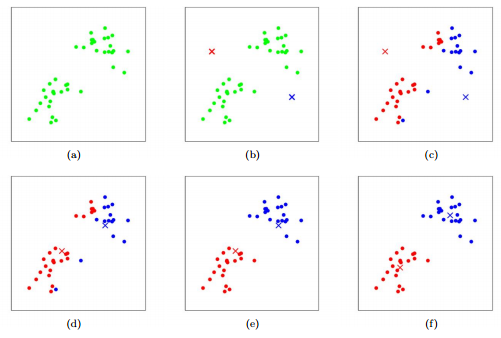
\includegraphics[scale = 0.8]{Figures/kmeans.png}
	\caption{Iterative steps for k-means}
	\label{fig: kmeans}
\end{figure}

\subsection{Outline}
Mathematically, the steps above can be written as:
Given a dataset $D = \bigl\{x_t\bigr\}^n_{t=1}$ and fix a number of clusters $1 \leq k \leq n$, we want to minimize the cost function 
\begin{equation*}
J = \sum_{j=1}^k \sum_{x \in D_j} \lVert x-\mu_j \rVert ^2
\end{equation*}
This cost function is the \textit{similarity measure} between our data. 
$D$ is partitioned into $D_1, D_2, \cdots, D_k$

\begin{itemize}
	\item Step 0 Initialize the centroids $\mu_{j}^{(1)}, j = 1,\cdots,k$ randomly 
	
	\item Step $l \in \mathbb{N}$ (E-step) Assign each point $x_t$ to its closest centroid, \begin{equation}\label{eq:3.1}
	j_t = \operatorname*{arg\,min}_{j=1,\cdots,k} \lVert x_t-\mu_j^{(l)} \rVert ^2
	\end{equation}
	\item Step $l \in \mathbb{N}$ (M-step) Recompute centroids, 
	\begin{equation}\label{eq:3.2}
	\mu_{j}^{(l+1)} = \frac{1}{\bigl\|\bigl\{t:j_t=j \bigr\}\bigr\|}\sum_{t:j_t=j} x_t
	\end{equation}
\end{itemize}

Remark: After E-step, we have a partition of $\bigl\{1,\cdots,n\bigr\}$, 
\begin{equation*}
D_j^{(l)}=\bigl\{t=1,\cdots,n,j_t^{(l)}=j\bigr\},\; \mu_j^{(l+1)} = \frac{1}{\bigl\|D_j^{(l)}\bigr\|}\sum_{t \in D_j^{(l)}}x_t
\end{equation*}

\subsubsection{K-means ++}
%D.arthur and S.vassilvitskii. kmeans++: the advantage of careful seeding. in proceedings of the eighteenth annual ACM-SIAM symposium on Discrete Algorithms, pages 1027-1035. Society for Industrial and Applied Mathematics, 2007).

K-means can sometimes result in bad clusterings or slow convergence if the initial centroids are chosen poorly. One way to address this issue is to run the k-means algorithm multiple times on a dataset and choose the best performing model in terms of the \textit{sum of squared errors}. Another strategy is to place the initial centroids far away from each other via the k-means++ algorithm \cite{Arthur2007}, which leads to better and more consistent results than the classic k-means.

The initialization in k-means++ can be summarized as follows:
\begin{itemize}
	\item Initialize an empty set $M$ to store the $k$ centroids being selected.
	\item Randomly choose the first centroid $\mu^{(j)}$ from the input samples and assign it to $M$.
	\item For each sample $x^{(i)}$ that is not in $M$, find the minimum squared distance $d(x^{(i)}, M)^2$ to any of the centroids in $M$.
	\item To randomly select the next centroid $\mu^{(p)}$, use a weighted probability distribution equal to $\frac{d(\mu^{(p)},M)^2}{\sum_i d(x^{(i)},M)^2}$
	\item Repeat steps 2 and 3 until $k$ centroids are chosen.
	\item Proceed with the classic k-means algorithm.
\end{itemize}

\subsubsection{Challenges}
One problem that \textit{k-means} has is that it gives slightly different clusters when it is run repeatedly for time-series data. As such, it is difficult to determine which run is the optimum.
%----------------------------------------------------------------------------------------

\section{Hierarchical Clustering} \label{4.4}
%add more citation \causton
Hierarchical Clustering can be divided into two: divisive and agglomerative. Here, we will discuss more on agglomerative hierarchical (HAC) which has also been extensively used to cluster gene expression values \cite{Eisen14863}. 

\subsection{Outline}
The algorithm starts from the trivial clustering that has each data point as a single-point cluster. Then, repeatedly, it merges the "closest" clusters of the previous clustering, as shown in Figure \ref{fig: hac}. Consequently, the number of clusters decreases with each such round. If kept going, it would eventually result in the trivial clustering in which all of the domain points share one large cluster. We then need to choose two parameters to define such an algorithm clearly: the distance (similarity measure or linkage) between clusters and stopping criterion for merging. The most common linkage measures are:
\begin{itemize}
	\item \textbf{Single}: between-clusters distance is defined by the minimum distance between members of the clusters, namely: $D(A,B) = \min \{d(x,y): x \in A, y \in B\}$
	\item \textbf{Average}: between-clusters distance is defined to be the average distance between a point in one of the clusters and a point in the other, namely:\\ $D(A,B) = \frac{1}{|A||B|}\sum\limits_{x \in A, y \in B}d(x,y)$
	\item \textbf{Max / Complete}: between-clusters distance is defined by the maximum distance between their elements, namely: $D(A,B) = \max \{d(x,y): x \in A, y \in B\}$
	\item \textbf{Ward}: this involves Ward variance minimization algorithm that deals with an error function. The error function is the average distance of each data point in a cluster to the centroid in the cluster. Between-clusters distance is defined as the error function of the unified cluster minus the error functions of the individual clusters.
\end{itemize}

\begin{figure}[h] 
	\centering
	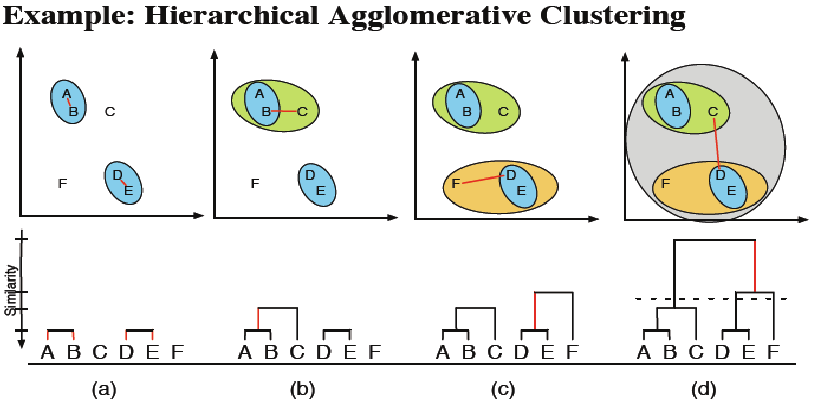
\includegraphics[scale = 0.5]{Figures/hierarchical_clustering.png}
	\caption{Iterative steps for hierarchical agglomerative clustering}
	\label{fig: hac}
\end{figure}
 
\subsection{Challenges}

Unlike other clustering methods, hierarchical clustering does not have any principled way to determine the optimal number of clusters. Thus, we have to determine which of the subtrees are clusters, and which subtrees are only a part of a bigger cluster. If one wishes to turn a dendrogram (lower part of Figure \ref{fig: hac}) into a partition of the space (a clustering), one needs to employ a \textit{stopping criterion}. Common stopping criterions include:
\begin{itemize}
	\item Fixed number of clusters: fix some parameter, $k$, and stop merging clusters as soon as the number of clusters is $k$.
	\item Distance upper bound: fix some $r \in \mathbb{R^+}$. Stop merging as soon as all the between-clusters distances are larger than $r$. We can also set $r$ to be $\alpha \max \{d(x,y): x,y \in \mathbb{X} \}$ for some $\alpha <1$. In that case the stopping criterion is called "scaled distance upper bound."
\end{itemize}

The second stopping criterion basically suggests that we want to stop merging when the cost of merging increases a lot and thus it most likely loses a lot of structure. As such, this leaves us to decide how big a merging cost is acceptable and there is no proven theory to say that this method will often or even usually lead to good choices. In addition, we may also face difficulty in picking the right similarity measure (or linkage) for our data.

%----------------------------------------------------------------------------------------

